% % % % % % % % % % % % % % % % % % % % % % % % % % % % % % % % % % % % % % % % %
\section{Die Bibliothek free-theorems}
% % % % % % % % % % % % % % % % % % % % % % % % % % % % % % % % % % % % % % % % %

Die Generierung freier Theoreme ist geradlinig und unkompliziert. Gerade deshalb ist es jedoch mühselig, diese Arbeit jedes
Mal per Hand durchzuführen, da ja immer die gleichen Schritte durchgeführt werden. Von daher ist es wünschenswert, diesen
Prozess zu automatisieren, und genau das macht die Bibliothek \textit{free-theorems} \cite{freetheorems}. Diese Bibliothek
beinhaltet die Werkzeuge, die nötig sind, um freie Theoreme aus Haskell-Programmcode zu generieren.

In diesem Kapitel wird näher darauf eingegangen, welche Werkzeuge dies sind und wie sie zusammenspielen. Es wird erläutert,
welche Schritte notwendig sind, um aus Quellcode eine Formel herzuleiten, die das entsprechende freie Theorem beinhaltet.
Abgeschlossen wird diese Übersicht dann mit einem kleinen Beispiel.

%In \cite{freetheorems} wird eine Implementierung vorgestellt, die die automatisierte Generierung von freien Theoremen aus
%Haskell-Code ermöglicht und die Grundlage darstellt, auf die die vorliegende Arbeit aufbaut.
%Sie erlaubt das Parsen von Haskell-Code, das Herausfiltern der entsprechenden Definitionen und deren relationale
%Interpretation, um schließlich die freien Theoreme zu erzeugen.
%Beigefügte Pretty printing Funktionen für Haskell-Syntax und Theoreme vereinfachen schließlich deren Darstellung.

%Im folgenden Abschnitt wird erläutert, wie diese Bibliothek grundlegend aufgebaut ist, wobei auf jeden einzelnen Schritt genauer
%eingegangen wird.


% - - - - - - - - - - - - - - - - - - - - - - - - - - - - - - - - - - - - - - - - - - - - - - - - - - - - - - - - - - - - - - - - - - - - - - - - - - - - - -
\subsection{Aufbau}
% - - - - - - - - - - - - - - - - - - - - - - - - - - - - - - - - - - - - - - - - - - - - - - - - - - - - - - - - - - - - - - - - - - - - - - - - - - - - - -

Die Bibliothek lässt sich grundsätzlich in drei Teile untergliedern: Frontend, Core und Pretty Printer \cite{freetheorems}. Die
Teile werden in dieser Reihenfolge durchlaufen \todo{vgl abbildung}.

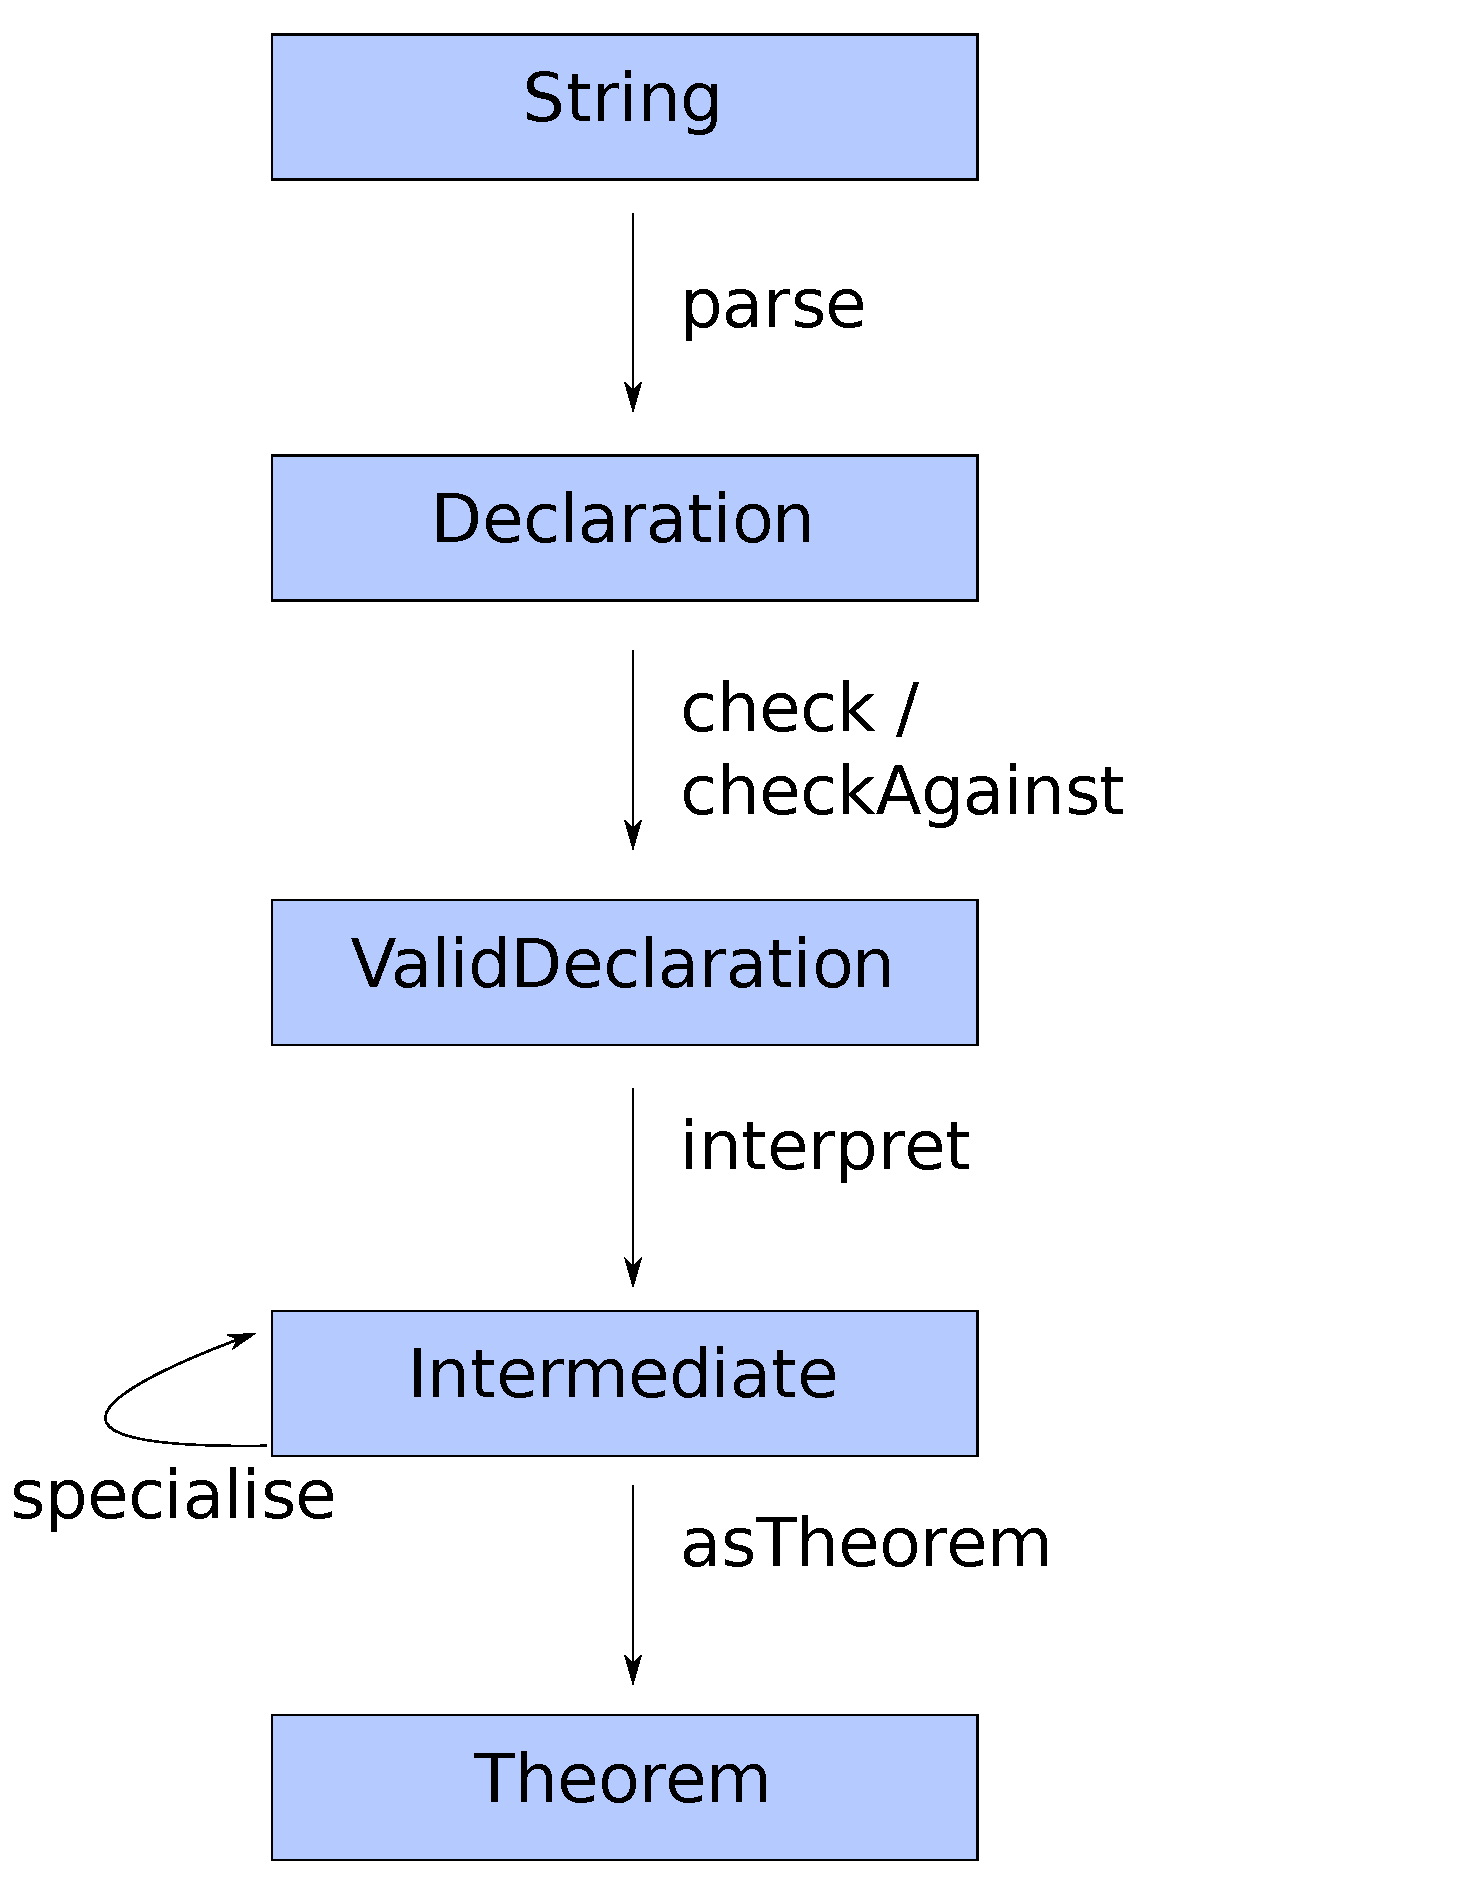
\includegraphics[height=300px]{overview-free-theorems}

Das Frontend ist der Teil, der den Haskell-Code entgegennimmt. Hier wird zunächst der Programmcode geparst und in einen
abstrakten Syntaxbaum übersetzt. Außerdem ist das Frontend dafür zuständig, Fehlerprüfungen durchzuführen und
ungültige Definitionen herauszufiltern, bevor der Syntaxbaum dann weiter an den Core gegeben wird.

%Zunächst werden im Frontend Parser bereitgestellt, um den Haskellcode aus einer Zeichenkette in eine passende Syntaxbaumstruktur umzuwandeln. Mithilfe einer check-Funktion
%wird diese Datenstruktur auf Gültigkeit überprüft, insbesondere in Bezug auf spezielle Anforderungen, die an die Definitionen gestellt wird, um Theoreme zu generieren.

Im Core findet dann die eigentliche Arbeit statt: Hier wird der Syntaxbaum in die entsprechende Relationaldarstellung
überführt und in eine Zwischendarstellung abgelegt, \texttt{Intermediate} genannt. Im nächsten Schritt wird diese
Relationaldarstellung dann Schritt für Schritt abgerollt und in eine Formel überführt. Diese Formel wird dann zurückgegeben.

Um diese Formel darzustellen, werden dann im Pretty Printer Teil entsprechende Funktionen bereitgestellt, die in der Lage
sind, den Formel-Datentypen in Zeichenketten umzuwandeln.

%\texttt{interpret} ist dann schließlich die Funktion, die eine Signatur in Bezug auf die anderen Deklarationen in eine Zwischendarstellung \texttt{Intermediate} überträgt. Die
%Funktion \texttt{asTheorem} entfaltet diese Darstellung \todo{``entfaltet''?} schließlich und überträgt sie in den Datentyp \texttt{Theorem}.


% - - - - - - - - - - - - - - - - - - - - - - - - - - - - - - - - - - - - - - - - - - - - - - - - - - - - - - - - - - - - - - - - - - - - - - - - - - - - - -
\subsection{Parser}
% - - - - - - - - - - - - - - - - - - - - - - - - - - - - - - - - - - - - - - - - - - - - - - - - - - - - - - - - - - - - - - - - - - - - - - - - - - - - - -

Um zu einer in Haskell geschriebenen Funktionssignatur irgendetwas zu generieren, muss zunächst eins getan werden: Aus dem
Programmcode muss die notwendige Information herausgezogen werden, der Haskell-Code muss geparst werden.
\textit{free-theorems} erfindet hier das Rad nicht neu sondern setzt auf einen Haskell-Parser, der mit \texttt{haskell-src-exts}
bereits als Paket verfügbar ist \cite{haskellsrcexts} \todo{cite} (bzw. \texttt{haskell-src} als Version, die keine
Spracherweiterungen unterstützt).

Dieses Paket bietet einen Parser für den kompletten Sprachumfang von Haskell inklusive aller Spracherweiterungen, die GHC
unterstüzt \cite{xyz} \todo{cite}. Der Parser liefert eine eigene Datenstruktur für einen abstrakten Syntaxbaum, aber der
enorme Sprachumfang hat natürlich zur Folge, dass dieser Syntaxbaum sehr komplex werden kann. Nun werden aber gar nicht
sämtliche syntaktischen Möglichkeiten der Sprache benötigt, ganz im Gegenteil: Für die Generierung freier Theoreme spielen
hauptsächlich Typsignaturen eine Rolle. Die Implementierungen, die in einem typischen Programm den Großteil des Programms
ausmachen, können getrost vernachlässigt werden.

Aus diesem Grund führt \textit{free-theorems} eine eigene Syntaxbaum-Datenstruktur ein und überführt den Syntaxbaum,
der von \texttt{haskell-src-exts} generiert wird, in eine vereinfachte Darstellung, genannt \texttt{BasicSyntax}.

%Neben dem Haskell 98 Parser, der keine \todo{Keine?} Spracherweiterungen zulässt, ist auch der Hsx Compiler gegeben, der die
%komplette Sprache mitsamt Spracherweiterungen umsetzt. Hier ist anzumerken, dass das Paket free-theorems in seiner aktuellen Form
%nicht mit dem aktuellen Haskell-Compiler kompatibel war und einige Anpassungen gemacht werden mussten. \todo{Evtl im Anhang Näheres?}
%Intern nutzt free-theorems hier die Pakete \texttt{Language.Haskell.Parser} bzw. \texttt{Language.Haskell.Exts.Parser}, die an sich bereits voll funktionstüchtige Parser liefern.

%Allerdings ist der komplette Sprachumfang sehr komplex und ein Arbeiten mit den Datenstrukturen, die von diesen genutzten Parsern generiert werden,
%wird unnötig erschwert. Aus diesem Grund transformiert free-theorems diese Datenstruktur in eine eigene, vereinfachte Struktur namens BasicSyntax. In dieser Struktur
%werden lediglich Typsignaturen festgehalten, Implementierungen werden vollkommen ignoriert, da sie für die Theoremgenerierung keine Rolle spielen.


\subsubsection{BasicSyntax}
% `````````````````````

Ein paar kleine Beispiele sollen ein Gefühl dafür vermitteln, wie der \texttt{BasicSyntax}-Datentyp aussieht. Dabei ist jeweils
eine Funktionssignatur gegeben und dahinter die Haskell-Darstellung des resultierenden BasicSyntax-Ausdrucks.

\begin{listing}[ht]
\inputminted[tabsize=2]{haskell}{ast.hs}
\caption{Beispiel}
\label{lst:ast}
\end{listing}

Listing \ref{lst:ast} zeigt die Datenstruktur am Beispiel \texttt{test :: [a] $\rightarrow$ [a]}. Die \texttt{parse}-Funktion des Parser-Moduls von \textit{free-theorems} liefert eine Liste sämtlicher relevanter Definitionen als \texttt{BasicSyntax} zurück.
In diesem Beispiel ist nur eine Typsignatur gegeben, \texttt{parse} gibt also eine einelementige Liste zurück, bestehend aus
genau einem Konstruktor \texttt{TypeSig}.

Da man freie Theoreme aus den Typsignaturen von Funktionen herleitet, könnte man sich überlegen, dass man auf alles andere
als Typsignaturen verzichten kann und der Rest des Programms irrelevant ist. Während dies für Implementierungen der Funktionen,
also die jeweiligen Funktionsrümpfe, zutrifft, gibt es dennoch andere Deklarationen, an denen man ebenfalls interessiert ist.

Man bekommt nämlich genau dann ein Problem, wenn der Entwickler im Programm eigene Datentypen deklariert und diese in
den Funktionssignaturen verwendet. Neben Funktionssignaturen werden also zusätzlich auch Datentypdeklarationen benötigt.
Hierzu gehören sowohl die \texttt{data}- als auch \texttt{type}- und \texttt{newtype}-Deklarationen (die semantischen Unterschiede
zwischen diesen verschiedenen Deklarationen spielen dabei keine Rolle). Listing \ref{lst:ast-data} zeigt ein Beispiel für eine
\texttt{data}-Deklaration und deren entsprechende Darstellung als \texttt{BasicSyntax}.

An diesem Beispiel kann man ebenfalls sehen, dass die Konstruktorparameter in die \texttt{Unbanged}-Struktur eingebettet sind.
Es gibt \texttt{Unbanged} und \texttt{Banged}, was einfach sagt, ob eine Striktheitsannotation vor dem entsprechenden
Parameter steht oder nicht. Es soll hier nicht näher darauf eingegangen werden, wozu diese Annotation verwendet wird, in
Kapitel \ref{sec:striktheit-und-rekursion} wird noch ein bisschen näher darauf eingegangen.

Klassendeklarationen werden insbesondere in Kapitel \ref{sec:erweiterung-um-typklassen} benötigt. Sie werden aber auch schon
von \texttt{free-theorems} beachtet und in die \texttt{BasicSyntax} mit aufgenommen. Der Grund dafür ist der, dass ja auch
Typvariablen in Typsignaturen auftreten können, die auf eine bestimmte Klasse eingeschränkt sind. Die aus der Allquantifizierung
resultierenden Relationen dürfen also nicht über alle Typen quantifiziert sein, sondern nur über solche, die zur entsprechenden
Klasse passen.

%Natürlich ist man hauptsächlich an den Funktionssignaturen interessiert, da man aus diesen die Theoreme ableitet. Aber natürlich können diese Signaturen ihrerseits wiederum 
%selbst definierte Datentypen oder auch Klasseneinschränkungen enthalten. Man kommt also nicht umhin, auch diese mit einzubeziehen und ebenfalls in der BasicSyntax vorzusehen.
%Das Beispiel in Listing \ref{lst:ast-data} zeigt eine data-Deklaration.

\begin{listing}[ht]
\inputminted[tabsize=2]{haskell}{ast2.hs}
\caption{Beispiel}
\label{lst:ast-data}
\end{listing}


% - - - - - - - - - - - - - - - - - - - - - - - - - - - - - - - - - - - - - - - - - - - - - - - - - - - - - - - - - - - - - - - - - - - - - - - - - - - - - -
\subsection{check}
% - - - - - - - - - - - - - - - - - - - - - - - - - - - - - - - - - - - - - - - - - - - - - - - - - - - - - - - - - - - - - - - - - - - - - - - - - - - - - -

\label{sec:check}

Im zweiten Schritt wird die \texttt{check}-Funktion benutzt, um alle Deklarationen auf Gültigkeit zu überprüfen und die Liste der Deklaration zu filtern. Ungültige Deklarationen
werden unter Angabe einer Fehlermeldung aus der Liste entfernt \cite{freetheorems}.

Es ist zwar davon auszugehen, dass die Syntax des Programmes korrekt ist, da ansonsten der Haskell-Parser bereits im ersten Schritt einen Fehler gemeldet hätte, dennoch ist
dieser zweite Schritt nötig, um auch korrekte Semantik voraussetzen zu können \todo{wahrscheinlich falsch ausgedrückt} (da andernfalls auch für fehlerhafte Programme Theoreme generiert würden, was keinen Sinn macht).

Die check-Funktion untergliedert sich in lokale und globale Checks, wobei die lokalen Checks pro Definition durchgeführt werden, die globalen Checks beziehen sich auf die Gesamtheit aller Definitionen. Beispielsweise wird lokal überprüft, ob bei Deklarationen die freien Variablen auf der rechten Seite auf der linken Seite der Defintion deklariert sind, es wird sichergestellt
dass auf der linken Seite alle Variablennamen verschieden sind, primitive Datentypen nicht deklariert werden usw.

Unter die globalen Checks fällt z.B., dass zu einem Funktionsnamen nicht mehrere Deklarationen existieren, dass alle Typkonstruktoren die korrekte Anzahl an Parametern haben oder auch dass keine Kreise in der Typklassenhierarchie existieren \cite{freetheorems}.

Am Ende schließt \texttt{check} noch alle Typausdrücke, dh. bei frei vorkommenden Typvariablen werden entsprechende Typabstraktionen um den Ausdruck geschlossen. Das ist wichtig, da in der weiteren Implementierung davon ausgegangen wird, dass alle Typausdrücke geschlossen sind und entsprechende Typabstraktionen zu jeder implizit allquantifizierten Variable vorhanden sind.

Tabelle \ref{bla} zeigt eine Übersicht aller globalen Überprüfungen.

\begin{tabular}{| l | l |}
\hline
Name&Beschreibung\\
\hline
  checkUnique&\\
  checkArities&\\
  checkAcyclicTypeSynonyms&\\
  checkAcyclicTypeClasses&\\
  checkAllConsAndClassesDeclared&\\
\hline
\end{tabular}


% - - - - - - - - - - - - - - - - - - - - - - - - - - - - - - - - - - - - - - - - - - - - - - - - - - - - - - - - - - - - - - - - - - - - - - - - - - - - - -
\subsection{interpret}
% - - - - - - - - - - - - - - - - - - - - - - - - - - - - - - - - - - - - - - - - - - - - - - - - - - - - - - - - - - - - - - - - - - - - - - - - - - - - - -

Tatsächlich macht die \texttt{interpret}-Funktion nichts, was nicht schon bekannt ist \todo{Das heißt, wenn ich es denn schon geschrieben hätte}: Sie überführt die Funktionssignatur in eine
Relationsdarstellung, wobei sie Typvariablen neu generierte Relationsvariablen zuordnet. Um es mit der Aufteilung von \cite{freetheorems} auszudrücken, stellt sie den Übergang des Frontends zum Core dar, wo der interessante Arbeitsschritt ausgeführt wird.

Der Datentyp, der hier verwendet wird, heißt Immediate. Dieser Datentyp ist letztlich nur ein Container für eine Relation mit
dem repräsentierten Typausdruck, zusätzlichen (unendlichen) Listen von freien Variablennamen und sonstigen Zusatzinformationen.


\subsubsection{Relation}
% ``````````````````

Für die Darstellung als Relationen definiert free-theorems den Datentyp \texttt{Theorem}, der folgende Konstruktoren hat:

\todo{unvollständig. und evtl unnötig}

\begin{tabular}{| l | l | l |}
\hline
Konstruktor & Parameter & Entsprechung \\
\hline
RelVar & RelationVariable & $\alpha$ \\
FunVar & (Either Term Term) & ? \\
RelBasic & - & R \\
RelLift & TypeConstructor [Relation] & [R], etc. \\
RelFun & Relation Relation & $S \rightarrow T$ \\
RelFunLab & Relation Relation & $S \rightarrow T$ \\
RelAbs & RelationVariable (TypeExpression,  & $\forall R . F R$ \\
& TypeExpression) [Restriction] Relation & \\
FunAbs & ... & \\
\hline
\end{tabular}

Wie man sieht, fehlt noch ein Konstruktor für die neu eingeführte Variante, dass eine Typkonstruktorvariable auf Relationen
angewandt wird. Darauf wird in Abschnitt \ref{sec:erweiterung-typklassen} eingegangen.


% - - - - - - - - - - - - - - - - - - - - - - - - - - - - - - - - - - - - - - - - - - - - - - - - - - - - - - - - - - - - - - - - - - - - - - - - - - - - - -
\subsection{asTheorem}
% - - - - - - - - - - - - - - - - - - - - - - - - - - - - - - - - - - - - - - - - - - - - - - - - - - - - - - - - - - - - - - - - - - - - - - - - - - - - - -

Die \texttt{asTheorem}-Funktion stellt eine Datenstruktur des Typs \texttt{Intermediate} als Theorem dar. Tatsächlich passiert hier aber eine ganze Menge mehr als der Name
vermitteln mag. Das schrittweise Abrollen der Relationen stellt schließlich den entscheidenden Schritt dar, durch den man überhaupt auf
die Theoreme schließen kann.

\todo{Hier eventuell auch ein Beispiel?}


% - - - - - - - - - - - - - - - - - - - - - - - - - - - - - - - - - - - - - - - - - - - - - - - - - - - - - - - - - - - - - - - - - - - - - - - - - - - - - -
\subsection{Spezialisieren von Relationsvariablen zu Funktionen}
% - - - - - - - - - - - - - - - - - - - - - - - - - - - - - - - - - - - - - - - - - - - - - - - - - - - - - - - - - - - - - - - - - - - - - - - - - - - - - -

Ist das Theorem generiert, kann man nun die Funktionsrelation spezialisieren, um das Theorem zu vereinfachen. Aus einem
$A : S \leftrightarrow T$ wird also $\forall a : S \rightarrow T$

usw.


% - - - - - - - - - - - - - - - - - - - - - - - - - - - - - - - - - - - - - - - - - - - - - - - - - - - - - - - - - - - - - - - - - - - - - - - - - - - - - -
\subsection{simplify}
% - - - - - - - - - - - - - - - - - - - - - - - - - - - - - - - - - - - - - - - - - - - - - - - - - - - - - - - - - - - - - - - - - - - - - - - - - - - - - -

Schließlich bietet free-theorems noch die Möglichkeit, die generierten Theoreme zu vereinfachen, indem nach einigen typischen
Mustern gesucht wird, beispielsweise: Entfernen aller unbenutzten allquantifizierten Variablen, $\forall v. f v == g v \rightarrow f == g$ usw.


% - - - - - - - - - - - - - - - - - - - - - - - - - - - - - - - - - - - - - - - - - - - - - - - - - - - - - - - - - - - - - - - - - - - - - - - - - - - - - -
\subsection{Beispiel}
% - - - - - - - - - - - - - - - - - - - - - - - - - - - - - - - - - - - - - - - - - - - - - - - - - - - - - - - - - - - - - - - - - - - - - - - - - - - - - -

In den vorangegangenen Abschnitten wurde ein kurzer Umriss der Bibliothek free-theorems gegeben, die im Folgenden um
Typkonstruktorklassen erweitert werden soll. Bevor die benötigten Änderungen erläutert werden, soll hier zunächst ein
kompletter Durchlauf als Beispiel gegeben werden. Es werden sämtliche Daten betrachtetet, die auf dem Weg von einer
Eingabezeichnekette zur resultierenden Ausgabezeichenkette entstehen.

\todo{Grafik}

Wir bemühen wieder unser Beispiel aus der Einleitung:

\begin{minted}{haskell}
f :: [a] -> [a]
\end{minted}

Im ersten Schritt setzt man einen bereitgestellten Parser ein, um diesen Haskell-Code in den bibliotheksinternen, vereinfachten
Syntaxbaum \texttt{BasicSyntax} zu parsen. Die \texttt{parse}-Funktion gibt genaugenommen eine Liste von \texttt{Declaration}s, also Deklarationen. Dabei handelt es sich um alle Toplevel-Deklarationen, die eine Rolle spielen, also Funktionssignaturen,
Datentypdeklarationen und Klassendeklarationen.

\begin{minted}{haskell}
...
\end{minted}

Hier wurde die Darstellung ein wenig vereinfacht, um das Verständnis zu erleichtern. Zu beachten ist aber, dass sämtliche
Funktionsimplementierungen wegfallen. Sie spielen für die Generierung freier Theoreme keine Rolle, das bedeutet aber auch,
dass free-theorems keine Fehlerprüfungen im Implementierungsteil durchführt. Die Bibliothek kann ohne Auftreten von Fehlern
durchlaufen, selbst der zu einer Funktionssignatur gehörige Code Fehler enthält.

Jetzt, da die \texttt{BasicSyntax} der Beispielfunktion vorhanden ist, muss \texttt{check} aufgerufen werden, um Fehler
zu entdecken. Ein Aufruf macht aus der Liste von \texttt{Declaration}s eine Liste von \texttt{ValidDeclaration}s. Tatsächlich
enthält diese Datenstruktur lediglich ein zusätzliches Feld \texttt{isStrictDeclaration}, das anzeigt, ob die entsprechende
Deklaration strikte Elemente enthält oder von diesen abhängt.

Um genau zu sein, ist der Ergebnistyp von \texttt{check} monadisch, es werden per Writer-Monade Fehlermeldungen
generiert, falls Fehler auftreten. Es ist noch anzumerken, dass \texttt{check} auch beim Auftreten von Fehlern eine Liste
von Deklarationen zurückgibt. Lediglich die Deklarationen, die Fehler enthalten, werden weggelassen; das bedeutet, dass
unter Umständen Theoreme generiert werden können, wenn nur Fehler auftreten, die keine Auswirkung auf das zu generierende
Theorem haben.

\begin{minted}{haskell}
...
\end{minted}

An dieser Stelle haben wir eine Liste gültiger Deklarationen, und wir haben eine Liste eventell aufgetretener Fehler. Um nun
freie Theoreme zu einer Typsignatur zu generieren, wird zunächst einmal eine Typsignatur benötigt. free-theorems bietet die
Funktion \texttt{filterTypeSignatures}, um Typsignaturen aus einer Liste von \texttt{ValidSignature}s herauszufiltern, was in
unserem Beispiel keinen Unterschied macht, weil es lediglich aus einer Typsignatur besteht.

Jetzt können wir \texttt{interpret} verwenden, um zu unserer \texttt{ValidSignature} unter Verwendung der übrigen
\texttt{Declaration}s die Relationaldarstellung unsereres Datentyps